 \addtolength\abovedisplayskip{-1\baselineskip}%
  \addtolength\belowdisplayskip{-1\baselineskip}%
  
\begin{tikzpicture}
\node[draw,very thick,rectangle,minimum width = \textwidth] (data) {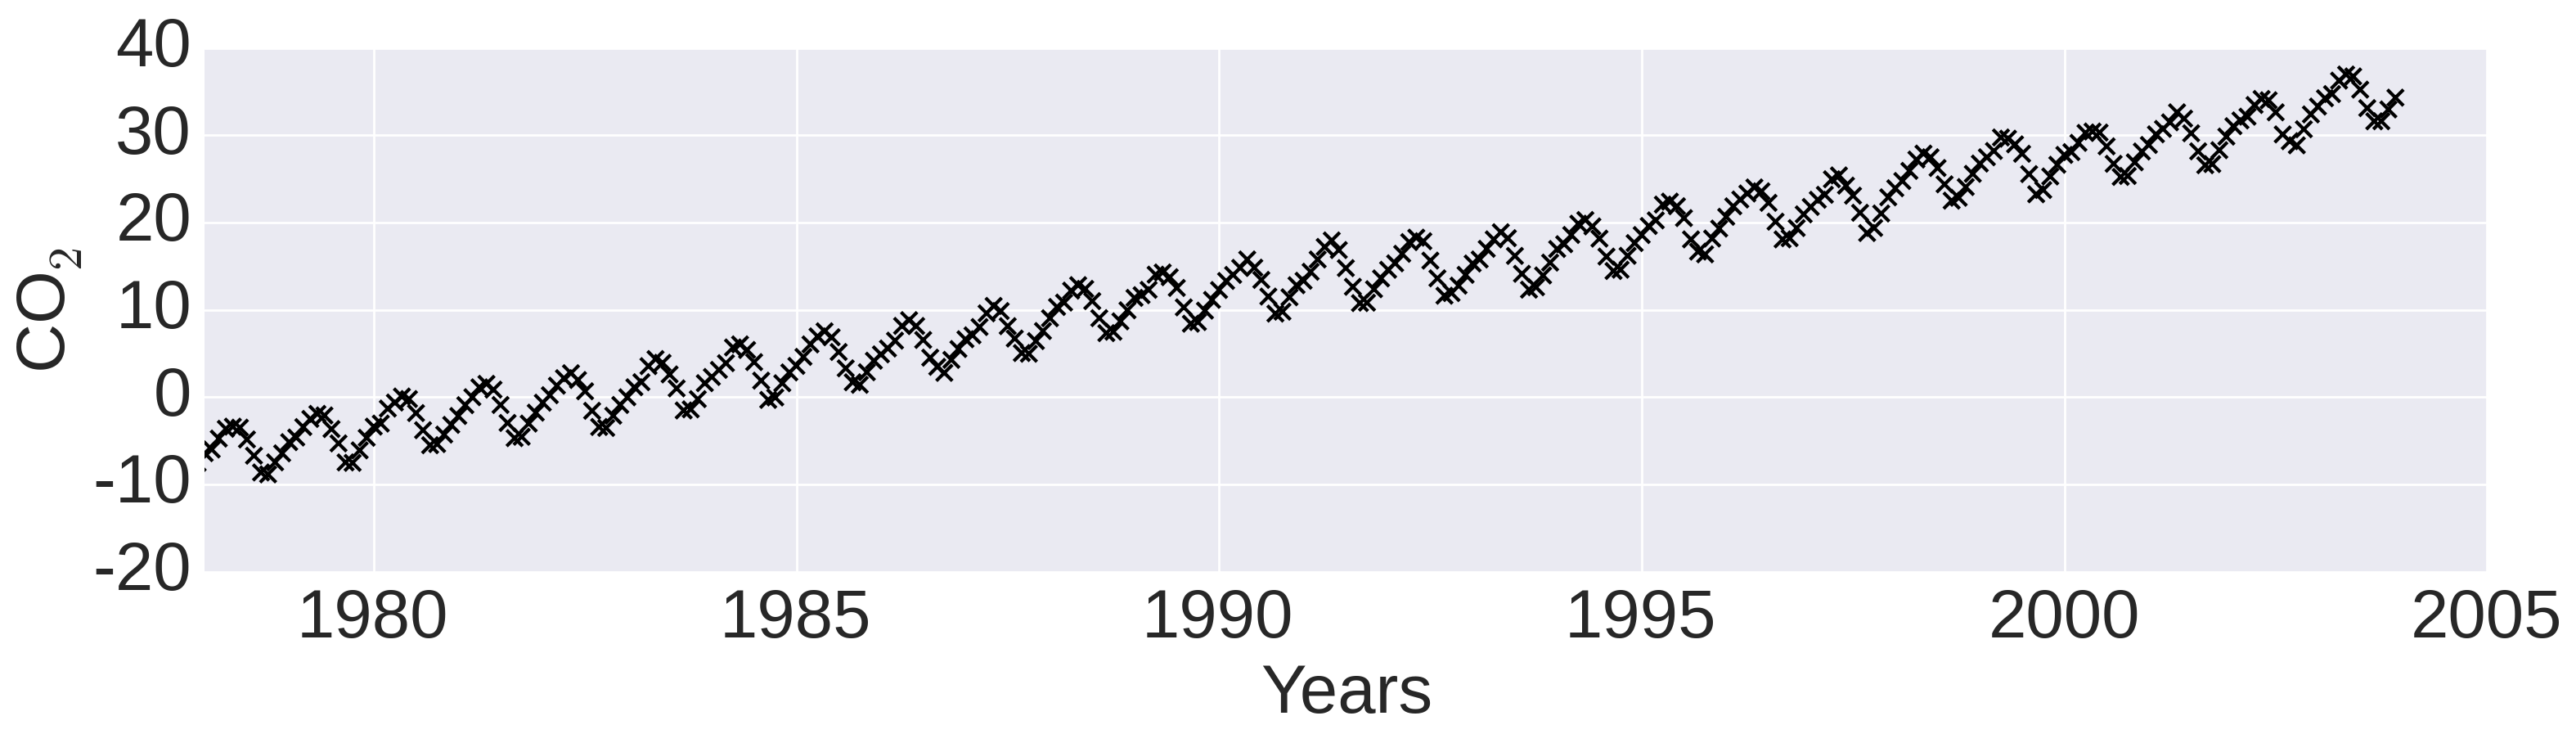
\includegraphics[width=0.9\textwidth]{figs/mauna_data.png}};
\node[below = 1.1cm of data, xshift=2cm] (posterior) {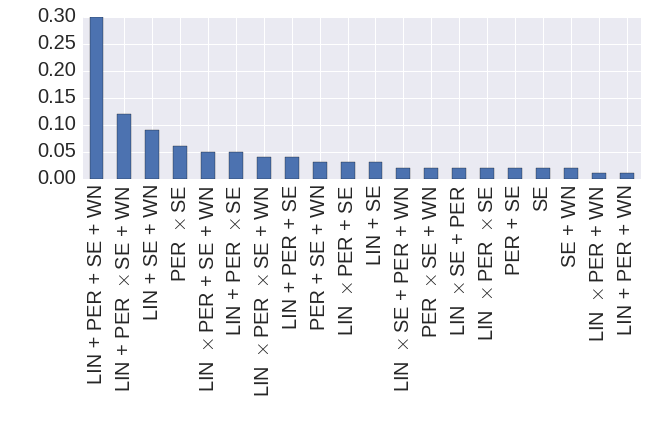
\includegraphics[width=0.7\textwidth]{figs/mauna_structure.png}};
\node[draw,rectangle,color=myblue,left = 0.cm of posterior,text block, text width = 3.6cm,minimum height = 6.5cm] (paragraph){\color{black}\footnotesize {\bf Qualitative Interpretation}:
The the posterior peaks at a kernel structure with four additive components. Additive components hold globally, that is there are no higher level, qualitative aspects of the data that vary with the input space. The additive components are as follows:\begin{itemize}[leftmargin=*]
 \item a linearly increasing function or trend;
 \item a periodic function;
 \item a smooth function; and
 \item white noise.
\end{itemize}
}; 
\node[draw,rectangle,color=myblue,below = 8.5cm of data] (formula) {\color{black}
$\mathbf{K}=\text{LIN} + \text{PER} + \text{SE} + \text{WN}$};
\node[draw,rectangle,color=myblue,below = 0.7cm of formula] (formula_param_1) {\color{black}
$= 2.7^2(x x^\prime) + 5.6^2 \exp \bigg( \frac{2 \sin^2 ( \pi (x - x^\prime)/3.7}{6.4^2} \bigg)
+ 0.4^2 \exp(-\frac{(x-x^\prime)^2}{2 \times 6.3^2}) +  1.9^2 \delta_{x,x^\prime} \label{eq:WN}$ };


\node[draw,rectangle,color=myblue,below = 0.7cm of formula_param_1] (post_param) {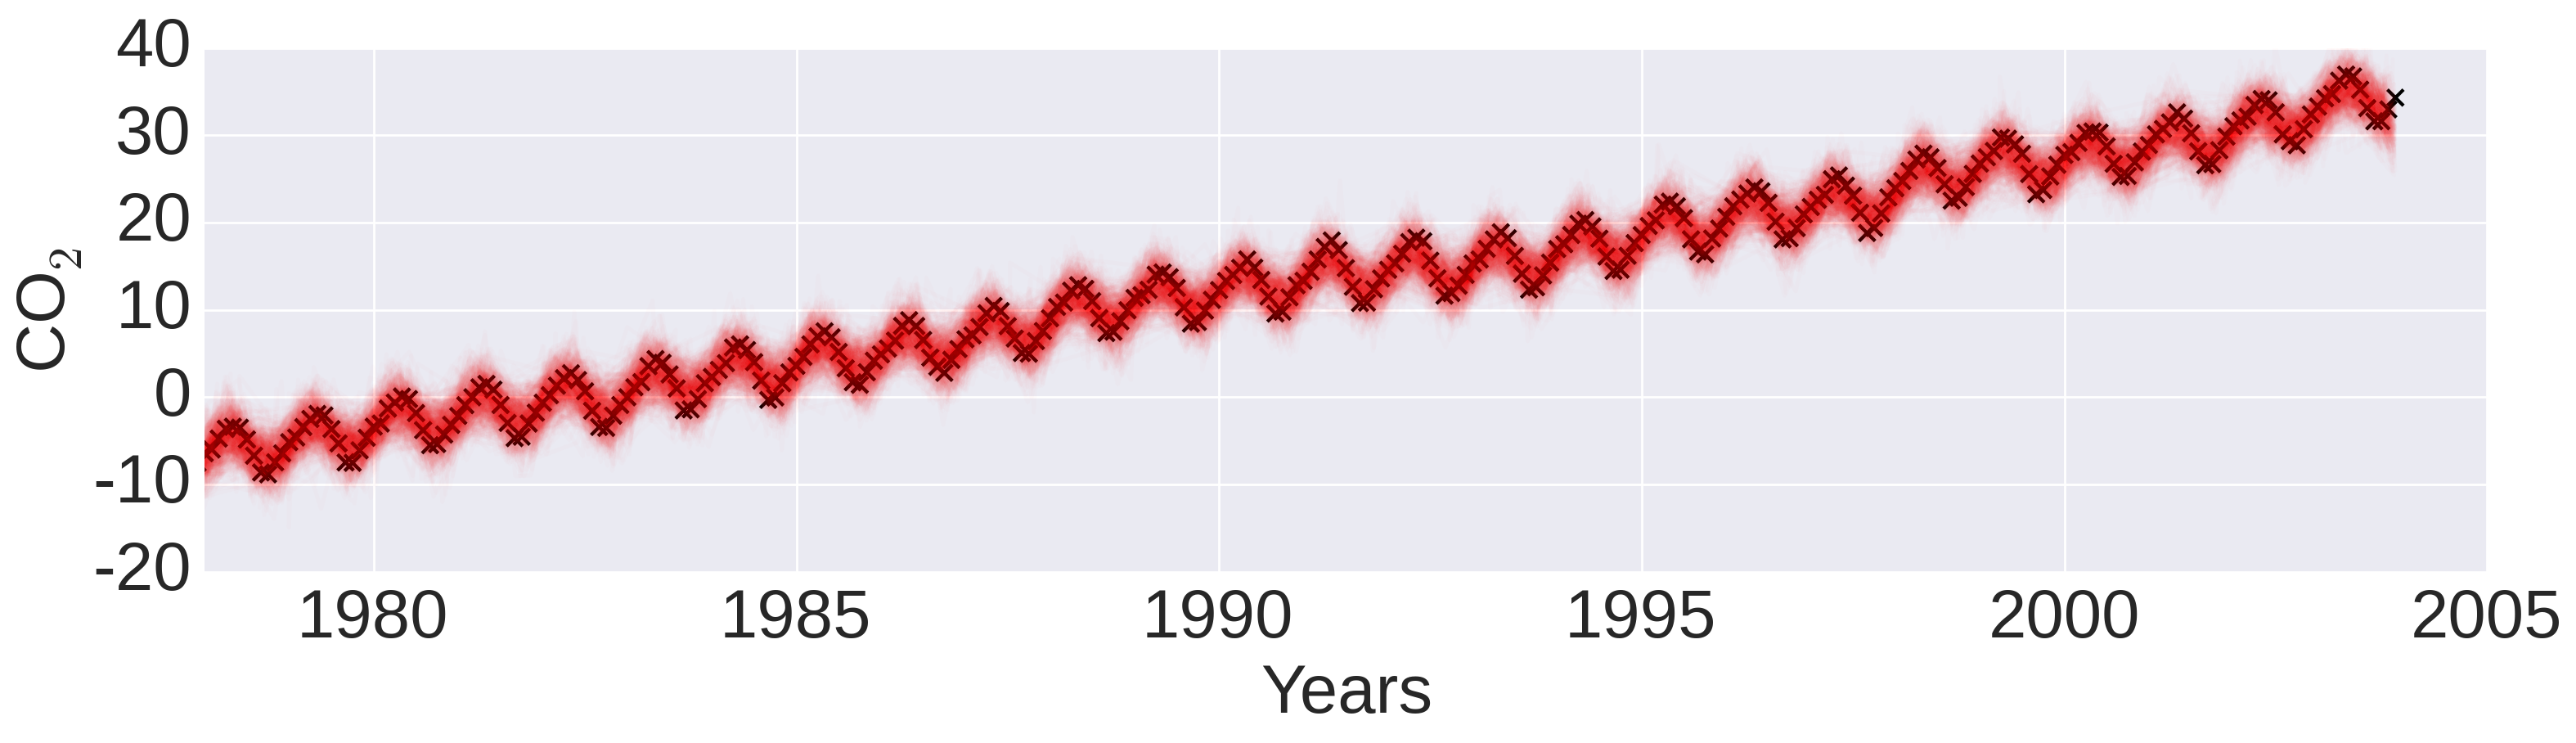
\includegraphics[width=0.8\textwidth]{figs/mauna_sample_1.png}};



\node[draw, rectangle,dashed,color=myblue, below = 1.4cm of data,minimum width = 0.45cm, minimum height = 5.8cm,xshift=-1.45cm] (mark_structure) {};
\node[draw,very thick, rectangle, below = 1.1cm of data,minimum width = \textwidth, minimum height = 15cm] (posterior_frame) {};

\node[left = 1.3cm of mark_structure] (paragraph_helper){};
\node[below =0.6cm of mark_structure,inner sep = 0pt,outer sep=0pt] (formula_helper) {};
\node[above =0.6cm of formula,inner sep = 0pt,outer sep=0pt] (formula_helper_2) {};

\draw[-,dashed,color=myblue] (mark_structure.south) -- (formula_helper);
\draw[-,dashed,color=myblue] (formula_helper) -- (formula_helper_2);
\draw[->,dashed,color=myblue] (mark_structure) -- (paragraph_helper);
\draw[->,dashed,color=myblue] (formula_helper_2) -- (formula);

\draw[->,color=myblue] (formula) -- (formula_param_1);
\draw[->,color=myblue] (formula_param_1) -- (post_param);

\draw[->,line width=1pt,double distance=2pt] (data) -- (posterior_frame);
\end{tikzpicture}
\addtolength\abovedisplayskip{1\baselineskip}%
\addtolength\belowdisplayskip{1\baselineskip}%


